\section{KiWi Algorithm}
\label{sec:alg}

KiWi implements a concurrent ordered key-value map supporting atomic (linearizable) \code{get(key)}, \code{put(key,value)}, and \code{scan(fromKey,toKey)} operations.
Its put operations are lock-free, whereas get and scan are wait-free. A put with a non-existent key creates a new KV-pair, and a put of the $\bot$ value removes the pair if the key exists.

The philosophy behind KiWi is to serve client operations quickly, while deferring data structure optimizations to a
maintenance procedure that runs infrequently. The maintenance procedure, \emph{rebalance}, balances KiWi's layout so as to ensure fast
access, and also eliminates obsolete information.

In Section~\ref{sec:organization}  we explain how data is organized in KiWi.   Section~\ref{sec:ops} discusses how the different operations are implemented atop this data structure in the common case, 
when no maintenance is required.
Section~\ref{sec:rebalance} focuses on rebalancing.


\subsection{Data organization}
\label{sec:organization}

\paragraph{Chunk-based data structure.}
Similarly to a B$^{+}$tree, the KiWi data structure is organized as a collection of large blocks of contiguous key ranges, called \emph{chunks}. Organizing data in such chunks allows memory allocation/deallocation to occur infrequently. It also makes the design cache-friendly and appropriate for NUMA, where once a chunk is loaded to local memory, access time to additional addresses within the chunk is much shorter. This is particularly important for  scans, which KiWi seeks to optimize, since they access contiguous key ranges, often residing in the same chunk.

The KiWi data layout is depicted in Figure~\ref{fig:overview-new}, with one chunk zoomed in.
The chunk data stucture is described in Algorithm~\ref{alg:chunk}.

\begin{figure*}[t]
  \centering
  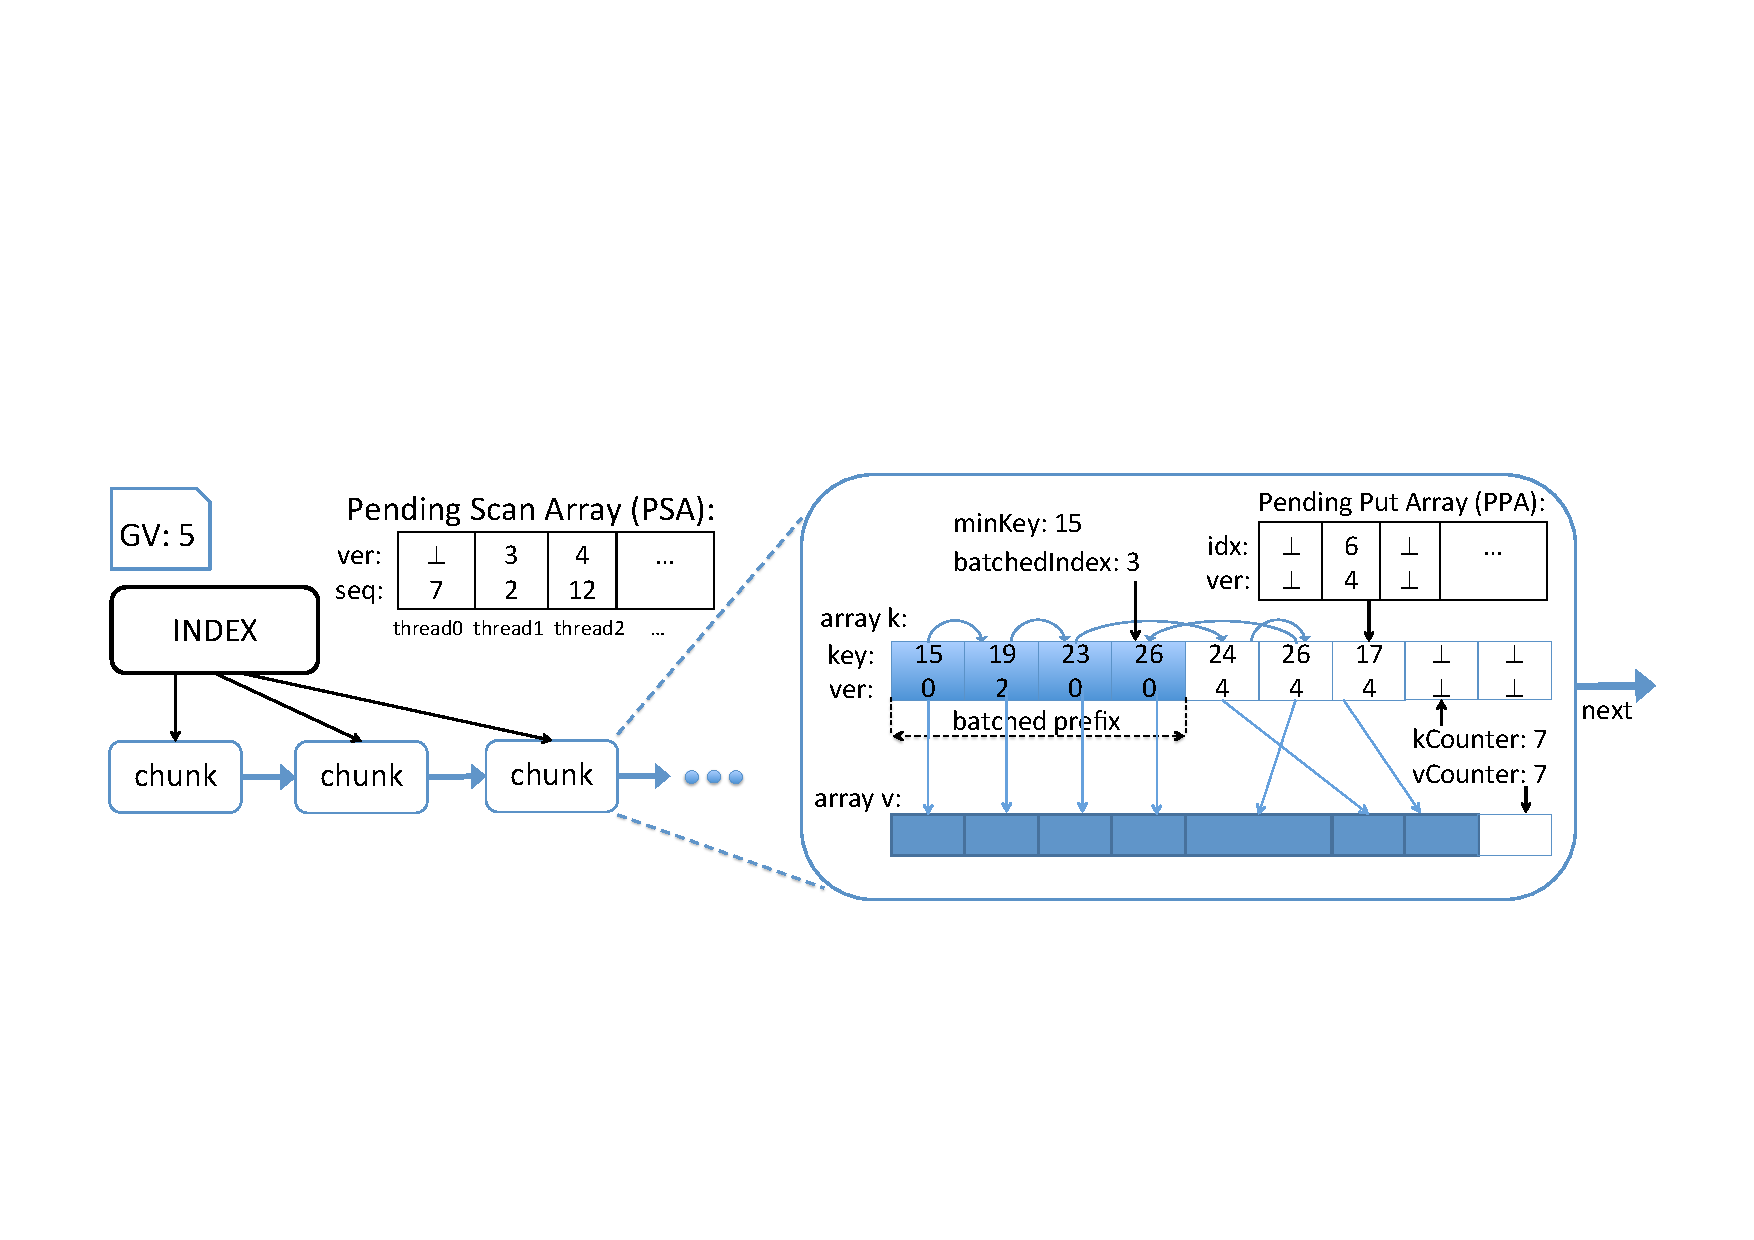
\includegraphics[width=.8\linewidth]{kiwi-layout4.pdf}
  \caption{{{\kiwi} data structure layout. In the zoomed in chunk (on the right), a pending put by the second
thread is attempting to add \code{k[6]} to the linked list with key $17$ and version $4$.}}
  \label{fig:overview-new}
\end{figure*}

\begin{algorithm}[t]
\codesize
\begin{center}
\begin{algorithmic}
%	\State \code{status}	\Comment{infant, normal, or frozen}
	\State immutable \codeF{minKey}  \Comment{minimal key in chunk}
	\State array \codeF{k} of $\langle$key, ver, valPtr, next$\rangle$    \Comment{in-chunk linked list}
	\State array \codeF{v} of values									\Comment{values stored in the list}
	\State \codeF{kCounter, vCounter} \Comment{end of allocated (full) prefixes} % in k and v
	\State \codeF{batchedIndex} \Comment{end of batched prefix in k}
\LineComment pending put array allowing scans and gets to help puts
	\State array \codeF{ppa[{\scshape num\_threads}]} of $\langle$ver, idx$\rangle$
	\State \codeF{next} \Comment{pointer to next chunk in chunk list}
	\State rebalance data $\langle$status, parent, ro$\rangle$ \Comment{rebalancing-related data}
\vspace{-1em}
\end{algorithmic}
\end{center}
\caption{{\kiwi} chunk data structure.}
\label{alg:chunk}
\end{algorithm}


KiWi's chunks are under constant renewal, as the rebalance process removes old chunks and replaces them with new ones.
It not only splits (over-utilized) and merges (under-utilized) chunks as in a B$^{+}$Tree, but also improves their internal
organization, performs \emph{compaction} by eliminating obsolete data, and may involve any number of chunks.
%A \code{status} field in the chunk indicates whether the chunk is undergoing rebalancing, as explained in Section~\ref{sec:rebalance} below.
% an \emph{infant} still being initialized, is a \emph{normal} part of
%the data structure, or is \emph{frozen} for rebalancing purposes.

In order to simplify concurrency control, however, we do not organize chunks in a B$^{+}$tree, but rather in a sorted linked list. This eliminates the synchronization complexity of  multi-level splits and merges.  Yet, to allow fast access, we supplement the linked list with an auxiliary \emph{index} that maps keys to chunks; it may be organized in an arbitrary way (e.g., skip-list or search tree).
Each chunk is indexed according to the minimal key it holds, which is invariant throughout its lifespan. 
(The minimal key of the first chunk in the list is $-\infty$.)
The index supports a wait-free
lookup method that returns the indexed chunk mapped to  the highest key that does not exceed a given {key}. It further supports conditional updates, which are explained in Section~\ref{sec:rebalance}, as they are done only as part of the rebalance procedure. Such updates are lazy, and so
the index may be inaccurate. Therefore, the index-based search is supplemented by a traversal of the chunk linked list.



% Chunk arrays
\paragraph{Intra-chunk organization.}
Each chunk is organized as an array-based linked list, sorted in increasing key order.
KiWi chunks hold two arrays -- \code{v} with written values, and \code{k} with the linked list.
Each cell in \code{k} holds a key, a pointer \code{valPtr}
to a value in \code{v}, and the index of the cell in \code{k} that holds the next key in the linked list.
It also has a version number, as we explain shortly.
When a chunk is created (as a result of rebalancing), some prefix (typically one half) of each array contains data,
and the suffix consists of empty entries for future allocation.

% Batched prefix for efficient binary search
The chunk's full prefix is initialized as sorted, that is, the linked-list successor of each cell is the ensuing cell in \code{k}.
The sorted prefix is called the chunk's \emph{batched prefix}, and it can be searched efficiently using binary search.
As keys are added, the order in the remainder of the chunk is not preserved,
i.e., the batched prefix usually does not grow.
For example, when a key is inserted to the first free cell, it creates a \emph{bypass} in the sorted linked list, where some cell $i$ in the batched prefix
points to the new cell, and the new cell points to cell $i+1$.
We note that in case the insertion order is random, inserted cells are most likely to be distributed evenly in between the batched prefix cells, thus
creating fairly short bypasses.
Given that the prefix and the remainder are of similar sizes, the expected search time remains poly-logarithmic.
Nevertheless, in the worst-case, the search time is linear in the size of the remainder of the chunk.

In order to support atomic scans, KiWi employs \emph{multi-versioning}, i.e., sometimes keeps the old version of a key instead of overwriting it. To this end, KiWi maintains a \emph{global version}, \code{GV}, and tags each key-value pair with a version, \code{ver}. Versions of a key are chained in the linked-list in descending version order. The compaction process that occurs as part of rebalancing eliminates obsolete versions.
Unlike traditional multi-versioning, KiWi creates new versions \emph{only} as needed for ongoing scans.
%This reduces the storage overhead between compactions.
%More importantly,
This allows us to shift the overhead for version management  from updates, which are short and frequent, to scans, which are typically long and therefore much less frequent. Specifically, put operations continue to use the same version (overwriting previous values for written keys, if they exist) as long as no scan operation increases  \code{GV}.


\paragraph{Coordination data structures.}
KiWi employs two %bookkeeping 
data structures for coordinating different operations. 
A global \emph{pending scan array} (PSA) tracks versions used by pending scans for compaction purposes;
each entry consists of a version \code{ver} and a sequence number \code{seq}, as well as the scan's key range.
% in order to avoid ABA races.
A per-chunk \emph{pending put array} (PPA) maps each thread either to a cell in the chunk that the thread is currently attempting to put into and a corresponding version, or $\langle \bot,\bot\rangle$, indicating that the thread is currently not performing a put.
The purpose of the PPA will become evident below.

\subsection{KiWi operations}
\label{sec:ops}

Our algorithm makes use of atomic \emph{compare-and-swap} -- CAS(x,old,new),  \emph{fetch-and-increment} -- F\&I(x), and
\emph{fetch-and-add} -- F\&A(x,a) instructions for synchronizing access to shared data; all impose memory fences.
A pseudocode of \kiwi\ operations is given in Algorithm~\ref{alg:ops}.

\paragraph{Helping puts.}

The interaction between put and scan operations is somewhat involved. In a nutshell, a put uses the current value of \code{GV}, whereas a scan begins by atomically fetching-and-incrementing \code{GV}, causing all future puts to write larger versions than the fetched one. Scan then uses the fetched version, \code{ver}, as its scan time, i.e., it returns for each scanned key the latest version that does not exceed \code{ver}.

However,  a race may arise if
 \code{put(key,val)}  reads a global version equal to \code{ver} for its data and then stalls while a concurrent scan obtains \code{ver} as its scan time and continues to read \code{key} before the put writes \code{val} for \code{key} with  \code{ver}. In this example, \code{val} should be included in the scan (since its version equals the scan time), but it is not (because it occurs late).

We overcome this scenario by having scans \emph{help} pending puts assign versions to values they write. To this end, puts publish their existence in the PPA of the chunk where they write, whereas scans call \code{helpPendingPuts} in each chunk where they read, which 
checks the PPA  and helps any relevant pending put threads it encounters (lines~\ref{l:help-pending}--\ref{l:help-pending-end}).
The helping here is minimal -- it consists of a single CAS that assigns a version to the pending put (line~\ref{l:help-pending-end}).
For example, in Figure~\ref{fig:linearization}, the scan helps \code{put(k1,a)} by setting its version to the current global version, namely $8$.
This orders the put after the scan, so the scan may return the old value.


Since scans use version numbers in order to decide which puts they take into account, the  order of put operations is determined by the order of their versions.
%rather than by the time at which the written value is added to the linked list.
For consistency, gets also need to rely on version numbers.
When a \code{get(key)}  encounters a pending \code{put(key,v)}  with no version, it cannot simply ignore the written value, because the put might end up ordered earlier than the get.
Gets therefore call   \code{helpPendingPuts}  to help pending puts as scans do.
This is depicted in Figure~\ref{fig:linearization}, where the get must help \code{put(k2,b)} obtain a version, because ignoring it
would order the gets inconsistently with the version order that would later be
observed by the scan.
%\todo{Add cross-reference to proof.}


\begin{figure}[tb]
\centerline{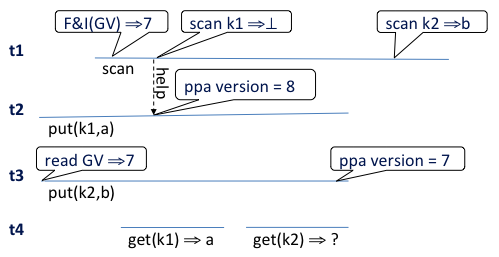
\includegraphics[width=0.85\columnwidth]{kiwi-linearization.png}}
\caption{Example of scan operation enforcing order between puts:
%according to version numbers:
The \code{scan} assigns
\code{put(k1,a)} a new version ($8$), whereas \code{put(k2,b)} later completes with an old version ($7$).
We see that if \code{get(k2)} does not help \code{put(k2,b)}, the gets see puts in a  different order than the  scan.
}
\label{fig:linearization}
\end{figure}

\paragraph{Put implementation.}


\begin{algorithm*}[tb]
\codesize
         \begin{multicols}{2}
	\begin{algorithmic}[1]{}

		\Procedure{put}{key, val}	
 \LineComment {\em 1. prepare cell to insert}
		\State locate target chunk $C$
\label{l:put-prep}
		\If{\codeF{checkRebalance($C$, \codeF{key, val}})}   \label{l:put-rebalance0}
			\State return \Comment{required rebalance completed the put}
		\EndIf
		\State \codeF{j} $\leftarrow$ F\&A($C$.\codeF{vCounter, val.size}) \Comment{allocate place for value}
		\State \codeF{i} $\leftarrow$ F\&I($C$.\codeF{kCounter}) \Comment{allocate cell in linked list}
		\If{ \codeF{j} $\geq$ \codeF{$C$.v.size} $\vee$  \codeF{i} $\geq$ \codeF{$C$.k.size}} 
			\If {$\neg$\codeF{rebalance($C$,\codeF{key, val})}} \codeF{put(key, val)}  \EndIf 
		\EndIf
		\State \codeF{v[j]} $\leftarrow$ \codeF{val}
		\State \codeF{k[i]} $\leftarrow \langle\codeF{key}, \bot, \codeF{j}, \bot\rangle$ \Comment{version and list connection not set yet}
\label{l:put-prep-end}
 \LineComment {\em 2. get version via PPA}
		\State \codeF{$C.$ppa[t].idx}  $\leftarrow$  \codeF{i}
\label{l:put-version}
		\State \codeF{gv} $\leftarrow$ \codeF{GV}      \label{l:put-LP}
		\State CAS($C.$\codeF{ppa[t]}, $\langle \bot$, \codeF{i} $\rangle$, $\langle$ \codeF{gv, i} $\rangle$) \label{l:put-cas-version}
		\If{\codeF{$C.$ppa[t].ver = frozen}} %%% or $C$.\codeF{status = frozen}}
		\Comment{$C$ is being rebalanced \label{l:put-frozen}}
			\If {$\neg$\codeF{rebalance($C$,\codeF{key, val})}} \codeF{put(key, val)}  \EndIf    		\label{l:put-restart}
		\EndIf
		\State  $C$.\codeF{k[i].ver}  $\leftarrow$   \codeF{$C.$ppa[t].ver}
\label{l:put-version-end}
 \LineComment {\em 3. add \codeF{k[i]} to linked list}
	\Repeat		
\label{l:put-ll}
		\State \codeF{c}$ \leftarrow$ \codeF{find(key, k[i].ver, $C$)} \Comment{search linked list $C.$\codeF{k}}
		\State						\Comment{use binary search up to $C.$\codeF{batchedIndex}}
		\If{\codeF{c} $= \bot$} \Comment{not found}
			\State link $C$.\codeF{k[i]} to the list using CAS \label{l:put-insert1}
			\If{CAS succeeded} break \EndIf
		\ElsIf{\codeF{c.valPtr} =  \codeF{j'}$<$\codeF{j}} \Comment{overwrite}
				\State  CAS(\codeF{c.valPtr, j', j}) \label{l:put-insert2}
		\EndIf		
	\Until{\codeF{c.valPtr} $ \geq$ \codeF{j}}
\label{l:put-ll-end}
%	\LineComment clean up
	\State  \codeF{ppa[t]} $\leftarrow \langle \bot, \bot \rangle$
\label{l:put-clean}
	\EndProcedure

\Statex
\Statex

	\Procedure{get}{key}	
		\State locate target chunk $C$ \label{l:get-start}
		\State \codeF{helpPendingPuts($C$, key, key)}
		\State return \codeF{findLatest(key, $\infty$, $C$)}
	\EndProcedure

\Statex

		\Procedure{scan}{fromKey, toKey}	
	 \LineComment {\em 1. obtain version - synchronize with rebalance via PSA}
		\State \codeF{psa[t]}  $\leftarrow$ $\langle ?$,\codeF{seq, fromKey, toKey}$\rangle$ \Comment{\codeF{seq} is a thread-local counter    \label{l:scan-version}}
		\State \codeF{ver} $ \leftarrow$ F\&I(GV)
		\State CAS(\codeF{psa[t]}, $\langle ?$,\codeF{seq, fromKey, toKey}$\rangle$, $\langle$\codeF{ver,seq, fromKey, toKey}$\rangle$)
			 \label{l:scan-FiCAS}
		\State \codeF{ver}  $ \leftarrow$  \codeF{psa[t].ver}
%%%  \Comment{accounts for the case that a version had already been assigned}
\label{l:scan-version-end}
	 \LineComment {\em 2. scan relevant keys}
		\ForAll{chunk $C$ in query range} \label{l:scan-scan}
			\State \codeF{helpPendingPuts($C$, fromKey, toKey)}
			\ForAll{key in query range}
				\State return \codeF{findLatest(key, ver, $C$)}
			\EndFor
		\EndFor \label{l:scan-scan-end}
%		\State \codeF{seq++} \label{l:scan-version}
		\State \codeF{psa[t]}  $\leftarrow$ $\langle\bot$,\codeF{seq++}$\bot, bot, \rangle$
	\EndProcedure

%\Statex
\Statex

	\Procedure{helpPendingPuts}{fromKey, toKey, $C$}  \label{l:help-pending}
			\ForAll {entry $e$ in $C$.\codeF{ppa}} 				
				\State \codeF{idx} $\leftarrow$ $e$.\codeF{idx} 
				\If{ $C$.\codeF{k[idx].key} $\in$ [\codeF{fromKey, toKey}]} 
					\State \codeF{gv} $\leftarrow$ \codeF{GV}  \label{l:get-readGV}
					\State CAS($e$, $\langle \bot$, \codeF{idx} $\rangle$, $\langle$ \codeF{gv, idx} $\rangle$)  \label{l:get-help}
					\label{l:help-pending-end}
				\EndIf
			\EndFor		
	\EndProcedure	

\Statex

	\Procedure{findLatest}{key, ver, C}  \label{l:find-latest}
%		\LineComment find cell in $C$ with \codeF{key} and highest version up to \codeF{ver} %, breaking ties using \codeF{valPtr}
		\State search \codeF{key} in $C$.\codeF{k} and \codeF{ppa}
% using binary search up to $C.$\codeF{batchedIndex} and then linear traversal	
%		\State search \codeF{key} in \codeF{ppa}
%		\If{found at least one cell with \codeF{key} and \codeF{ver}}
%			\State return  one with  highest \codeF{valPtr}
%		\EndIf
		\If{found at least one cell with \codeF{key} and version $\leq$\codeF{ver}}
			\State return one with highest version, break ties by \codeF{valPtr}
		\EndIf
	\State return $\bot$
	\EndProcedure	

	\algstore{kiwi} %% Uncomment to add another pseudocode figure
	\end{algorithmic}
	\end{multicols}
	\caption{\kiwi\ operations -- pseudocode for thread \code{t}.}
	\label{alg:ops}
\end{algorithm*}


The put operation appears in the left column of Algorithm~\ref{alg:ops}. It
consists of three phases: (1) locate the target chunk and
prepare a cell to insert with the written value; (2) obtain a version while syncrhonizing with
concurrent scans, gets, and rebalances via the PPA; and (3) connect  the new cell to the linked list.

%For simplicity we describe the algorithm as if both the key and value are embedded in the cell; in practice, to support variable length values the cell %can consist of pointer to where the value is stored.

The first phase (lines~\ref{l:put-prep}--\ref{l:put-prep-end})
locates the target chunk $C$, traversing the index and the linked list if needed. Later this phase allocates space for the key and the variable-length value, by increasing $C$'s array  counters to the next available indices \code{i} and \code{j} for \code{k} and \code{v}, resp.
This is done using atomic F\&I and F\&A, so in case of concurrent put operations, each thread gets its own cells.

Before increasing \code{i} and \code{j}, put checks if rebalancing is needed, because the chunk is full, imbalanced, or immutable, 
as discussed in the next section. This is done by the procedure \code{checkRebalance} given below, 
which returns \code{false} in case no rebalance is needed, and otherwise completes (or restarts) the put.
%, which restarts the put operation in case it needs to rebalance.  
After increasing \code{i} and \code{j}, put verifies that they are not too large, 
and if so, proceeds to write values into \code{k[i]} and \code{v[j]}, without a version at this point; note that \code{k[i]} is not yet connected to the linked list.

The second phase (lines~\ref{l:put-version}--\ref{l:put-version-end}) publishes \code{i} in the thread's entry in $C$'s PPA,
and then uses CAS to set the version to the current value of \code{GV}.
The CAS may fail in two possible ways. First, if the chunk is undergoing rebalancing, then
the reblanacing thread may have set the thread's PPA version to \code{frozen}.
In this case, the put cannot proceed since the chunk is deemed immutable. Instead, it invokes \code{rebalance}, 
and if rebalance returns false indicating that it did not insert the put's key and value, the put restarts
(lines \ref{l:put-frozen}--\ref{l:put-restart}).
(Invoking rebalance on a chunk that is already being rebalanced is done for lock-freedom, given that the original rebalancing thread
may be stalled.)
Second, a helping thread may have already set the version;
to account both for this case and for the case CAS succeeds,
put uses the version from the PPA, and copies it to \code{k[i]} (line \ref{l:put-version-end}).

The third phase, (lines~\ref{l:put-ll}--\ref{l:put-ll-end}), adds \code{k[i]} to the linked list.
To find the insertion point, it first uses binary search on the batched prefix and then traverses the remaining linked list.
If the linked list does not contain a cell with the same key and version, then \code{k[i]} is linked to the list (line \ref{l:put-insert1}).
Otherwise, ties between two puts with the same key and version are broken based on the indices of their allocated cells in \code{v}.
If the put that allocates cell \code{j} finds in the linked list a cell with index \code{j'} with the same key and version such that \code{j'}$<$\code{j},
it uses CAS to replace that cell's \code{valPtr} to point to \code{v[j]} (line \ref{l:put-insert2}).
If \code{j'}$>$\code{j} then the put does nothing, since its value has effectively been overwritten.
Note that in both cases some cell, either \code{j} or \code{j'}, remains allocated but is not connected to the linked list.
%Namely, at most one cell with a given key-version pair is connected to the linked list.
Unconnected cells are compacted by the  rebalancing process.
Finally, the PPA version is cleared (line \ref{l:put-clean}).
%using a CAS (line \ref{l:put-clean}).
%The CAS is used to account for a race with a concurrent rebalancing thread that attempts to set the version to \code{frozen}.

\paragraph{Gets and scans.}

Gets and scans are presented in the right-hand column in Algorithm~\ref{alg:ops}.
A \code{get(key)} begins by querying the index for \code{key}, and then (if needed), traverses the linked-list of chunks until
the next chunk's \code{minKey} exceeds \code{key} (line \ref{l:get-start}).
If there is a pending put to \code{key} that does not have a version yet, (i.e., its version is $\bot$), get attempts to help it by setting its version to
the current value of \code{GV} using CAS  (line \ref{l:get-help}). (CAS may fail in case the put sets its own version or is helped or frozen by another thread).
It then calls \code{findLatest()}  to find the latest version of the searched key.

The \code{findLatest()} function (line~\ref{l:find-latest}) performs a binary search on the batched prefix, and continues to traverse the in-chunk linked list until it either finds  \code{key} or finds that it does not exist. In addition, \code{findLatest()} checks the PPA for potential pending puts of the target key,
ignoring entries with no versions as these were added after the help.
In case multiple versions of \code{key} exist, it returns the one with the highest version.
If a pending put has the same version for the sought key as an entry in the linked list, then the one with the larger \code{valPtr} is returned.

A scan first determines its scan time  (lines \ref{l:scan-version}--\ref{l:scan-version-end}).  It obtains a  unique version via F\&I of \code{GV},
and attempts to set it as its scan time while synchronizing itself relative to helping rebalance operations
as described below.

It then reads all the keys in the relevant range (lines \ref{l:scan-scan}--\ref{l:scan-scan-end})
by traversing the list of chunks, and within each chunk, proceeding as get does to help all pending puts and find the latest version of each key.

\paragraph{Ordering operations.}



\begin{table}[t]
\codesize
\begin{center}
\begin{tabular}{|l|c|c|c|}

 \hline
 {\bfseries } 		& {\bfseries scan}			& {\bfseries put }    	& {\bfseries rebalance }	\\
 \hline

 {\bfseries scan}       & F\&I 	\codeF{GV}  	& \textendash				& \textendash			\\
% 				& \codeF{GV}     		& 						& 					\\
\hline
 {\bfseries put } 	& CAS		 		& by version, then	 		& \textendash			\\
 			        &  \codeF{ppa[t].ver} 		& F\&A \codeF{vCounter} 		& 				\\
\hline
 {\bfseries rebalance}& 	CAS				& CAS  to \codeF{frozen}   		& CAS \\
				& 	\codeF{psa[t].ver} 			& \codeF{ppa[t].ver}   		& \codeF{rebalanceObj} \\
 \hline

\end{tabular}
\end{center}
\caption{Atomic operations and rendevouz points determining order between \kiwi\ procedures.}
\label{tab:sync}
\end {table}

The  order among concurrently executing \kiwi\ procedures is determined by atomic hardware operations
(F\&I, F\&A, or CAS) on pertinent memory locations.
Table~\ref{tab:sync} summarizes the rendevouz points for different types of operations. For brevity, we omit gets from the table.

Each scan has a unique version. The order between concurrent scans is determined by
the order in which they (or the rebalance threads that help them) perform F\&I on \code{GV}.
Scans (and gets) order themselves relative to a put by thread \code{t} via \code{ppa[t].ver} in the chunk where the put occurs.

The order between puts that attempt to  insert the same key is determined by their versions, which reflects their order wrt ongoing scans.
Puts that have the same version, (i.e., the order between them is not determined by scans), are ordered according to
the order in which they succeed to fetch-and-add  \code{vCounter}.
Rebalance operations are discussed below.




\subsection{Rebalancing}
\label{sec:rebalance}

Section~\ref{sec:rebalance-trigger} discusses the life-cycle of a \kiwi\ chunk, and in particular,
when it is rebalanced. Section~\ref{sec:rebalance-stages} then walks through the stages of the rebalance process.

\subsubsection{Triggering rebalance and chunk life-cycle}
\label{sec:rebalance-trigger}

We saw that put calls \code{checkRebalance($C$)} in line~\ref{l:put-rebalance0} of Algorithm~\ref{alg:ops} before adding a new key to $C$.
This procedure triggers \code{rebalance($C$)} whenever $C$ is full or otherwise unbalanced, according
to some specified \emph{rebalance policy}; we refer to $C$ as the \emph{trigger chunk} of the rebalance.

To address the immediate problem, \kiwi\ could, in principle, restrict itself to the trigger chunk:
It can free up space by \emph{compacting} $C$, i.e., removing deleted values, values that are no longer in the linked list
because their keys have been over-written, as well as values that pertain to old versions that are not required by any active scan;
if this does not suffice (because all the information in $C$ is needed), \kiwi\ may \emph{split} the chunk.
Furthermore, it can address the imbalance  by \emph{sorting} the chunk.

The problem with this approach is that it may leave under-utilized chunks in the data structure forever.
\kiwi\ improves space utilization by allowing chunks to \emph{merge}, or more generally,
\emph{engaging} a number of old chunks in the rebalance,
and replacing all of them with any number of new ones.
The chunks to engage are determined by the rebalance policy.

Rebalance clones the relevant data from all engaged chunks  into new chunks, and then
replaces the engaged chunks with the new ones in the data structure.
Cloning creates a window when the same data resides at two chunks -- new and old.
In order for get and scan to be wait-free, the chunks remain accessible for reading during this period.
But in order to avoid inconsistencies, both chunks (old and new) are immutable throughout the window.

This defines a life cycle for chunks: they are created as immutable \emph{infants} by some \emph{parent} trigger chunk $C$;
they become \emph{normal} mutable chunks at the end of the rebalance process; and finally, they become \emph{frozen}
(and again immutable) when they are about to be replaced.
(We assume that a complementary garbage-collection mechanism eventually removes disconnected, frozen chunks.)
%after there are no pointers to them.
%from the chunk linked list, the index, or active threads.
The chunk's status (infant, normal, or frozen), the pointer to parent, and the pointer to rebalance object are part of the rebalance data
stored in the chunk (see Algorithm~\ref{alg:chunk}).


The \code{checkRebalance($C$)} procedure is given in Algorithm~\ref{alg:rebalance}. 
It checks whether $C$ is immutable, and if so, helps complete the process that makes it immutable
($C$'s parent in case $C$ is an infant, and $C$ in case it is frozen).
The rebalance procedure consists of two functions, \codeF{rebalance} and \codeF{normalize}; in case
the chunk's parent is helped only the latter is perfromed as explained below.
In addition, if the chunk is full or if the rebalance policy chooses to do so, it also triggers rebalance on $C$.
Note that put calls \code{checkRebalance} before incrementing \code{kCounter} and \code{vCounter} in order to avoid filling up infant chunks.
The \code{reblance} procedure takes the put's key and value as parameters, and attempts to piggyback the put on the reblanace, i.e., insert the key and value to the newly created chunk. In case it fails, it returns false, in which case the put is restarted. 

\begin{algorithm}[tb]
\codesize
	\begin{algorithmic}[1]{}
		\algrestore{kiwi} %% Uncomment to add another pseudocode figure
		\Procedure{checkRebalance}{$C$, key, val}
		\If{\codeF{$C$.status=infant}} 
			\State normalize($C$.parent)
			\State \codeF{put(key, val)} 
		\EndIf
		\If{\codeF{$C$.vCounter} $\geq$ \codeF{$C$.v.size} $\vee$ \codeF{$C$.kCounter} $\geq$ \codeF{$C$.k.size} $\vee$ 
			\State \codeF{$C$.status = frozen}  $ֿֿ\vee$ \codeF{policy($C$)} 
			} 
			\State ok $\leftarrow$ \codeF{rebalance($C$, key, val)}
			\State normalize($C$)
			\If {$\neg$ok} \codeF{put(key, val)} \EndIf 
		\EndIf
		\EndProcedure
		\algstore{kiwi} %% Uncomment to add another pseudocode figure
	\end{algorithmic}
\caption{The checkRebalance procedure.}
\label{alg:check-rebalance}
\end{algorithm}	


The  policy will typically choose to rebalance $C$ whenever $C$ is full or under-utilized, as well as when
its  batched prefix becomes too small relative to the number of keys in $C$'s linked list.
In order to stagger rebalance attempts in case of many insertions to the same chunk,
the policy can make probabilistic decisions:  If a chunk  is nearly full or somewhat under-utilized or
unbalanced, then the policy may flip a coin to decide whether to invoke rebalance or not.
%Of course, if the chunk already full, it needs to be rebalanced immediately.

\subsubsection{Rebalance stages}
\label{sec:rebalance-stages}

\newenvironment{compactenum}
{ \begin{enumerate}
    \setlength{\itemsep}{0pt}
    \setlength{\parskip}{0pt}
    \setlength{\parsep}{2pt}     }
{ \end{enumerate}      }

Rebalance  proceeds in the following seven stages:
\begin{compactenum}
\item \emph{Engage} -- agree on the list of chunks to engage.
\item \emph{Freeze}  -- make engaged chunks immutable.
\item \emph{Pick minimal version} --  to keep in compaction.
%, after helping pending scans obtain versions.
\item \emph{Build} -- create infant chunks to replace engaged ones.
\item \emph{Replace} -- swap new chunks for old ones in  list.
\item \emph{Update index} -- unindex old chunks,  index new ones.
\item \emph{Normalize} -- make the new chunks \emph{mutable}.
\end{compactenum}

If the first check of \code{checkRebalance()} decides to help rebalance a chunk's parent, then
rebalance starts in stage $6$, since the chunk's reachability implies that stage $5$ is complete.
In the other two cases, (a frozen chunk or a new trigger chunk), rebalance cycles through all seven stages.
This is safe because all stages are idempotent, and ensures lock-freedom, namely, progress in case the original rebalance stalls.
The first five stages are performend in the \codeF{rebalance} procedure, whereas the last two are performed in \codeF{normalize}.
\inote{A pseudo-code for the rebalance process is given in Algorithm~\ref{alg:check-rebalance}.
We now describe the stages in detail.}
%
For space limitations we omit the rebalance pseudocode; we now describe the seven stages.

\begin{algorithm*}[th]
\codesize
         \begin{multicols}{2}
	\begin{algorithmic}[1]{}
	\algrestore{kiwi}
	\Procedure{rebalance}{$C$, put\_key, put\_val}	
	\LineComment {\em 1. engage }
	\State \codeF{ro} $\leftarrow$ new rebalance object, initially $\langle C, C.\codeF{next}, \bot \rangle$
	\State \codeF{last} $\leftarrow C$
	\State CAS($C$.\codeF{ro}, $\bot$, \codeF{ro})
	\State \codeF{ro} $\leftarrow$ $C$.\codeF{ro}
	\While{ \codeF{ro.next} $\not=\bot$ }
		\State \codeF{next} $\leftarrow$ \codeF{ro.next}
		\If{\codeF{policy(next)}} \Comment{try to engage next}
		 	\State CAS(\codeF{next.ro}, $\bot$, \codeF{ro}) 
		 	\If{\codeF{next.ro = ro}}  \Comment{engaged next}
		 		\State CAS(\codeF{ro.next}, \codeF{next}, \codeF{next.next}) 
		 		\State \codeF{last} $\leftarrow$  \codeF{next}
			\Else 		 		
				\State  CAS(\codeF{ro.next}, \codeF{next}, $\bot$) 	
			\EndIf
		\Else 		 		
			\State  CAS(\codeF{ro.next}, \codeF{next}, $\bot$) 	
		\EndIf
	\EndWhile

	\LongLineComment {search the last concurrently engaged chunk}
	\ForAll{chunks \codeF{c} from \codeF{last} s.t. \codeF{c.ro} $=$ \codeF{ro}}
		\State \codeF{last} $\leftarrow$ \codeF{c}
	\EndFor

	\LineComment {\em 2. freeze}
	\State $C$.\codeF{status} $\leftarrow$ \codeF{frozen}
			\ForAll {entry $e$ in $C$.\codeF{ppa}} 				
				\State \codeF{idx} $\leftarrow e$.\codeF{idx} 
				\State CAS($e$, $\langle\bot$, \codeF{idx}$\rangle, \langle$\codeF{frozen, idx}$\rangle$)  
			\EndFor		

	\LineComment {\em 3. pick minimal version}

	\ForAll{\codeF{psa[t] = $\langle$?, seq, from, to$\rangle$}}
		\If{$C$.minKey $\le$ to $\wedge$ 
			\State $C$.next.minKey $>$ from} 
			\State add { $\langle$t, seq, from, to$\rangle$} to \codeF{toHelp}
		\EndIf
	\EndFor				
	\If{toHelp $\not=\emptyset$}
		\State \codeF{ver} $ \leftarrow$ F\&I(GV)
		\ForAll{$\langle$t, seq, from, to$\rangle \in$  \codeF{toHelp}}  
				\State CAS(\codeF{psa[t]}, $\langle$?,\codeF{seq,from,to}$\rangle, \langle$\codeF{ver,seq,from,to}$\rangle$)
		\EndFor
	\EndIf

	\vspace{10mm}
	\LineComment {\em 4. build}
	\LongLineComment{we assume the \# of versions is much smaller than the chunk size}
	\State $C_f \leftarrow C_n \leftarrow$ new chunk  
		\State \hspace{5mm} with \codeF{minKey}=$C$.\codeF{minKey}, \codeF{parent}=$C$, \codeF{status=infant} 
	\ForAll{chunks $C_o$ from \codeF{ro.first} to \codeF{last}}
		\If{$C_o$.\codeF{minKey} $<$ \codeF{put\_key} $<$ $C_o$.\codeF{next.minKey}}   
			\State  \codeF{toPut} $\leftarrow \{ \langle$\codeF{put\_key},GV, \codeF{put\_val}$\rangle \}$
		\Else
			\State \codeF{toPut} $\leftarrow \emptyset$
		\EndIf
		\ForAll{keys k in $C_o \cup $\codeF{toPut} in sorted order}
			\If{$C_n$ is more than half full} 
				\State $C_n$.\codeF{next} $\leftarrow$  new chunk 
					\State \hspace{5mm} with 
					\codeF{minKey}=$C$.\codeF{k}, \codeF{parent}=$C$, \codeF{status=infant} 
				\State $C_n \leftarrow C_n.$\codeF{next}
			\EndIf
			\ForAll{versions $\langle$ ver, val $\rangle$ of k, in descending order}
				\State insert $\langle$ k, ver, val $\rangle$ to $C_n$
				\If{ver $<$ \codeF{minKey}} break \EndIf
			\EndFor
		\EndFor
	\EndFor
	\LineComment {\em 5. replace}
	\State \codeF{last.immutable} $\leftarrow$ true
	\State $C_n$.\codeF{next} $\leftarrow$ \codeF{last.next}
	\State \codeF{pred} $\leftarrow$ $C$'s predecessor
	\If{CAS(\codeF{pred.next+immutable}, $C$+false, $C_f$+false)} 
		\State return true  \Comment{insertion succeeded}   \EndIf
	\If{\codeF{pred.next.parent} = $C$} 
		\State return false \Comment{someone else's insertion succeeded}
	\Else \Comment{insertion failed, help predecessor and retry}
		\State rebalance(pred, $\bot, \bot$)
		\State return rebalance($C$, put\_key, put\_val)
	\EndIf 

	\EndProcedure
	
	\Statex
	
	\Procedure{normalize}{$C$}	
	\LineComment {\em 6. update index}
	\ForAll{chunks $c$ from $C_f$ to $C_n$}
		\State load: \codeF{index.loadPrev($c$.minKey)}
		\If {$\neg c$.\codeF{frozen}}
			\If{$\neg$ \codeF{index.putConditional($c$.minKey, $c$)}}
				goto load 
			\EndIf 
		\EndIf
	\EndFor		
	\ForAll{chunks $c$ from \codeF{ro.first} to \codeF{last}}
			\State \codeF{index.deleteConditional($c$.minKey, $c$)}
	\EndFor
	\LineComment {\em 7. normalize}	
	\ForAll{chunks $c$ from $C_f$ to $C_n$}
		$c$.\codeF{status $\leftarrow$ normal}
	\EndFor		
	\EndProcedure

		\end{algorithmic}
	\end{multicols}
\caption{\kiwi's rebalance operation.}
\label{alg:rebalance}
\end{algorithm*}	

\paragraph{1. Engagement.}



Since multiple threads may simultaneously execute \code{rebalance($C$)}, they need to reach \emph{consensus} regarding
the set of engaged chunks. The consensus is managed via pointers from the chunks to a dedicated rebalance object \code{ro}.
Once a chunk is engaged in a rebalance it cannot be engaged with another rebalance.
The engaged chunks in a particular rebalance always form a contiguous sector of the chunks linked list.
For simplicity, this sector always starts from the trigger chunk forward,  though in principle it is possible
to grow the sector backwards from the trigger chunk as well.
A rebalance object holds pointers to three chunks, \code{first} (the trigger chunk) and \code{next} 
(the next potential chunk to engage in the rebalance).
%A rebalance object holds pointers to three chunks, \code{first}, \code{next} and \code{last}, where \code{first} is
%the trigger chunk,  \code{next} is the next potential chunk to engage in the rebalance,
%and \code{last} is the (agreed-upon) final chunk of the rebalance.
%, after all the nodes between the trigger chunk and it have been engaged.
The engagement  preserves the following invariant:
\begin{invariant}
Consider a rebalance object \code{ro}.
If \code{ro.next}${\not=}{\bot}$ then
for every chunk $C$ in the linked list from \code{ro.first} to the chunk before \code{ro.next}, \code{$C$.ro=ro}.
\end{invariant}


%Algorithm~\ref{alg:engage} includes pseudocode for engagement, which
Engagement
begins by agreeing on the \code{ro} to use. This is done by (1) creating a rebalance object
 referring to the trigger chunk $C$, (2) attempting to set \code{$C$.ro}
to the new rebalance object via CAS, and (3) using the \code{ro} in \code{$C$.ro}.
Note that the latter was set by a successful CAS of some rebalance thread.
Next, we try to engage ensuing chunks in the list one by one.
In each iteration, we consult the policy whether to engage the next chunk.
We then use CAS to change \code{ro.next} to either \code{ro.next.next}, or $\bot$ indicating
that it is time to stop engaging chunks.
We exit the loop when \code{ro.next} is $\bot$, and then set the local variable \code{last} 
to  the last engaged chunk.


\paragraph{2. Freezing.}

Once the list of engaged chunks is finalized, we freeze them so no data will be added to them
while they are being cloned. Recall that puts become visible to concurrent retrievals once they
publish themselves in the chunk's PPA, and that before doing so, they check if the chunk
is frozen. However, we need to account for the scenario where a chunk becomes frozen after
put checks its status and before the put publishes itself in PPA.
To this end,
rebalance traverses all PPA's entries and attempts to set their versions to frozen using CAS.
If the CAS is successful, the put will fail to assign itself a version
(Algorithm~\ref{alg:ops}, line~\ref{l:put-restart}). Otherwise, the put has already assigned its version, and
rebalance can take it into account during cloning.
\inote{
As an optimization, it is possible to help pending puts perform the actual linked-list insertion
in order to avoid the need to clone data from the PPA.
}

\paragraph{3. Determining the minimal read version and helping scans.}

We need to clone all data versions that might still be needed by scans.
To this end, we compute \code{minVersion}, the minimum read point among all active  and future scans --
this is the smallest version among those published in PSA and the current \code{GV}.

Since a scan cannot atomically obtain a scan time from \code{GV} and publish it in PSA,
rebalance cannot ignore scans that have started but did not publish a version yet.
We therefore use a helping mechanism: scan first publishes ? in PSA (Algorithm~\ref{alg:ops}, line~\ref{l:scan-version})
indicating its intent to obtain a version, then fetches-and-increments the global version
and uses CAS to update the version from ? to the one it obtained.

Concurrent rebalance operations help scans install a version in started entries;
monotonically increasing counters are used to prevent ABA races where an old rebalance ``helps'' a new scan.
Specifically, rebalance does the following: (1) it scans the  PSA for entries with ? whose range overlaps the
range covered by the engaged chunks; (2) if any are found, it fetches-and-increments \code{GV} and
reads its new version into \code{gv}; (3) for every \code{psa[t]}=  $\langle$?, $n \rangle$ entry found in (1),
it attempts to CAS \code{psa[t]} to  $\langle$\code{gv}, $n \rangle$.
Note that scan's CAS (line~\ref{l:scan-FiCAS})  might fail  in case it is helped, but
either way, it uses the version written by some successful CAS (line~\ref{l:scan-version-end}).


\paragraph{4. Creating new chunks and completing the put.}

The next stage creates new chunks to replace the engaged ones. It traverses the list of engaged chunks from \code{ro.first} to \code{last}.
In each chunk, it collects data both from the intra-chunk linked list and from the PPA. Additionally, 
the key and val of the put that triggered the rebalance is included in the appropriate chunk. 
All versions of a key that are older than the last version that does not exceed \code{minVersion} can be safely discarded, whereas
newer versions are cloned into new chunks. New chunks are created one at a time, as infants, with the trigger chunk as their parent.
%, and the intra-chunk linked list sorted.

Keys are added, in sorted order, to a new chunk $C$ until it is roughly half full, at which point a new chunk $C'$ is created
and $C.\code{next}$ is set to $C'$. (In case the last chunk is too sparse, for example, only a quarter full, it is discarded and its keys are moved to the  penultimate chunk).

\paragraph{5. Data structure update.}

Next, rebalance attempts to insert the new section into the linked list instead of the engaged one.
This involves two steps: First, the \code{next} pointer of the tail chunk in the new section needs to take the value of
the \code{next} pointer in \code{last}. Second, the \code{next} pointer of the predecessor of \code{ro.first} needs to be set to the head of
the new chunks' list. In order to execute the two steps atomically, we do the following:
(1) \emph{mark} the \code{next} pointer in \code{last} as immutable;
(2) set the tail of the new chunk sector to its value; and
(3) use CAS to set the \code{next} pointer of the predecessor of \code{ro.first}.

If CAS succeeds, we return true.
If CAS fails because another rebalance (using the same rebalance object) has successfully replaced the trigger chunk with a new one, we simply return false (indicating that the new key and value were not added as part of the rebalance, and hence put should restart) 
without taking any additional actions. But if CAS fails because some other rebalance had marked the \code{next} pointer as immutable (step (1) above), then we recursively help that rebalance complete, and then re-attempt to insert the new chunk sector to the list.

In the special case when the new list is empty (because no data is kept), step (3) CASes  the \code{next} pointer of the predecessor of \code{ro.first} to the  \code{next} pointer of \code{last}.

\paragraph{6. Index update.}

%The next phase adds the new chunks to the index and removes  the replaced ones.
Since the new chunks are already accessible via the linked list and the old chunks are already frozen, the index update can be lazy, and updates of different chunks can proceed without synchronization.
Nevertheless, we need to take into account races with old rebalance operations--- a thread that wakes up after being stalled must be prevented from indexing a chunk that had already been supplanted.

To this end, we assume that the index supports a form of semantic load-linked and store-conditional; specifically, it provides the following API:
(1) \code{loadPrev(k)} --- returns the indexed chunk mapped to the highest key that does not exceed \code{k};
(2) \code{deleteConditional(k,$C$)} --- removes key \code{k} only if mapped to chunk $C$; and
(3) \code{putConditional(k,prev,$C$)} --- maps \code{k} to $C$ provided that the highest key in the index that does not exceed
\code{k} is mapped to \code{prev}.
Such an index can be implemented in non-blocking ways using low-level atomic operations \cite{BraginskyP2012}; in our implementation,
we instead use locks.

To index a new chunk $C$, we first call \code{loadPrev($C$.minKey)}, then verify that $C$ is not frozen, and if so,
add it conditionally to the index. If the conditional put fails and yet the chunk is not frozen, the put is retried.
Index removals call \code{deleteConditional(C.minKey,C)}.

\paragraph{7. Normalization.}
Finally, the status of the new chunks is set to normal, and put operations may begin to update them.
Though it is possible that old (removed) chunks are still being accessed by old get and scan operations at this point, these operations will
be ordered before the new puts, so it is acceptable for them to miss the added data. Once all such old operations complete, the
old chunks can be reclaimed.

